% --------------------------------------------------------------------------
% Template for Project Course paper; to be used with:
%          ProjectCourse21.sty  - Project Course 2021 LaTeX style file, and
%
% --------------------------------------------------------------------------

\documentclass{article}
\usepackage{MAECapstoneCourse,amsmath,graphicx,url,times}
\usepackage{color}
\usepackage[utf8]{inputenc}
\pagenumbering{arabic}

% Example definitions.
% --------------------
\def\defeqn{\stackrel{\triangle}{=}}
\newcommand{\symvec}[1]{{\mbox{\boldmath $#1$}}}
\newcommand{\symmat}[1]{{\mbox{\boldmath $#1$}}}

% Title.
% --------------------
\title{Progressive Inference for Music Demixing}

\name{Giorgio Magalini, Alessandro Manattini, Filippo Marri}
\address{Dipartimento di Elettronica, Informazione e Bioingegneria (DEIB), Politecnico di Milano\\
Piazza Leonardo Da Vinci 32, 20122 Milano, Italy\\   
\tt{[giorgio.magalini,alessandro.manattini,filippo.marri]@mail.polimi.it}    
}

\begin{document}

\ninept
\maketitle

\begin{sloppy}

\begin{abstract}

Isolating individual sources from a musical mixture remains a key challenge in audio engineering, with wide-ranging applications from production to restoration. This work investigates whether a progressive inference strategy, inspired by diffusion models, can enhance the performance of an existing demixing network such as HDemucs. The proposed method iteratively refines the target stem by remixing the previous estimate into the original mixture using a scheduled weighting, and reapplying the separation at each step. As a preliminary validation, we demonstrate that increasing the relative gain of a stem in the mixture improves its separation quality—a lemma referred to as the “oracle predictor implication”—thereby justifying the progressive approach. The system is evaluated on the MUSDB18-HQ dataset using scale-invariant signal-to-distortion ratio (SI-SDR) as the metric, and tested under different update strategies and configurations. While early iterations show slight improvements for the target source, the performance plateaus and eventually declines, suggesting that fixed schedules and lack of model adaptation limit the effectiveness of the approach. The findings indicate that simply reusing a pre-trained separator in an iterative loop is insufficient, and that meaningful gains could be achieved by incorporating noise modeling, adaptive blending, and end-to-end retraining within a diffusion-based framework.

\end{abstract}

\begin{keywords}
Source separation, diffusion models, MUSDB18-HQ, HDemucs
\end{keywords}

\section{Introduction and Background}
\label{sec:intro}

Music demixing, also known as source separation, refers to the process of isolating individual instruments (i.e., drums, bass, vocals) from a single, fully mixed audio track. This task holds significant relevance in audio engineering, music production, and scientific research. Over time, numerous methodologies have been explored to address this challenge.

Among traditional approaches is Nonnegative Matrix Factorization (NMF), which decomposes a magnitude spectrogram into a product of basis and activation matrices. Concurrently, repetition-based techniques have gained traction for foreground/background separation in audio signals. These approaches capitalize on the repetitive nature of many musical accompaniments. REPET \cite{rafii2013repet} estimates a periodic background by averaging spectrogram frames spaced at a fixed interval. Its variants, including Adaptive REPET \cite{rafii2013repet}, which accommodates slowly changing periods, and REPET-SIM \cite{rafii2013repet}, which utilizes a spectral similarity matrix instead of strict periodicity, offer improved adaptability in handling non-stationary or intermittent audio patterns. Another conventional method, Harmonic-Percussive Source Separation (HPSS) \cite{hpss}, distinguishes percussive elements from harmonic content based on temporal characteristics.

Despite the utility of these classical techniques, recent advancements in deep learning have demonstrated superior performance. Traditional digital signal processing (DSP) approaches are grounded in explicit spectral or temporal assumptions, offering interpretability and computational efficiency. However, they often underperform when dealing with non-stationary harmonics, complex reverberation, or timbral masking. In contrast, modern machine learning (ML) models—ranging from convolutional neural networks (CNNs) to diffusion models—leverage large-scale datasets to learn non-linear, data-driven representations capable of capturing intricate sonic structures and dynamics.

Traditional DSP-based source separation is commonly classified as blind source separation. Machine learning, by contrast, derives substantial advantages from its training phase, enabling the model to extract patterns learned from data rather than relying on pre-defined heuristics. This learning-based paradigm is a key factor behind the improved performance of ML techniques over classical DSP methods.

A seminal ML-based approach to source separation emerged with the introduction of the U-Net architecture, originally developed by Ronneberger et al. \cite{Unet_medical_segmentation} in 2015 for biomedical image segmentation. The architecture is named for its characteristic U-shape, composed of a contracting path (encoder) that captures contextual information and a symmetric expanding path (decoder) that facilitates precise localization. A defining feature of U-Net is its skip connections, which link encoder and decoder layers at corresponding resolutions, preserving high-resolution features critical for accurate segmentation and reconstruction. Although originally intended for medical imaging, U-Net’s architecture has proven highly adaptable. In audio processing, music demixing can be analogized to segmenting different frequency components from a composite audio signal, making U-Net a natural fit for this task.

Subsequent advancements led to the development of the Demucs model. The early versions (v1 and v2) adopted a U-Net-based architecture that operated directly on raw waveforms, working entirely in the time domain \cite{Demucs}. These models learned to separate sources by analyzing the audio signal as it is perceived, with the initial layers implicitly performing a time-frequency decomposition via learned convolutions. A major innovation was introduced in Hybrid Demucs, which employs a dual-branch U-Net architecture. One branch processes the waveform in the time domain, while the other operates in the spectral domain via spectrograms \cite{HybridDemucs}. This hybrid configuration enables the model to harness the complementary advantages of both representations. The most recent version, Hybrid Transformer Demucs (HT Demucs) \cite{rouard2023hybrid}, incorporates a cross-domain Transformer encoder into the deepest layers of the U-Net. This design facilitates the fusion of spectral and temporal information, enabling the model to capture long-range dependencies and further enhancing separation quality.

More recently, generative modeling approaches—particularly diffusion models—have emerged as a powerful framework for source separation \cite{Karchkhadze2024Improving}. These models are trained to learn data distributions by progressively adding and then removing noise from input signals \cite{Karchkhadze2024Improving}. The denoising process is mathematically formalized as solving a probability flow ordinary differential equation (ODE) \cite{Karchkhadze2024Improving}, with a neural network estimating the score function that guides the denoising trajectory \cite{Karchkhadze2024Improving}. In practice, this involves iterative refinement of the extracted sources, analogous to polishing a noisy signal. This concept is readily applicable to music source separation.

Following the framework proposed by Karras et al. in \textit{Elucidating the Design Space of Diffusion-Based Generative Models} \cite{karras2022elucidating}, we adopt an iterative procedure in which each instrument stem is gradually extracted from the mixture. At each iteration, the neural network refines its output by conditioning on the previous extraction, mirroring the progressive denoising in diffusion models. In this analogy, the mixture corresponds to noise, and the extracted stem is the denoised target. This strategy enables a gradual and accurate reconstruction of individual sources from a complex mix.

\section{Methodology}
\label{sec:method}
To conduct the analysis, a jupyter notebook\footnotemark{} has been created whose code has been structured in a modular fashion in a way that by setting different parameters to a single function, several experiments can be conducted. \footnotetext{https://github.com/alessandromanattini/DEMIXING} This function takes as input the stems, it mixes them, it demixes the mixed track by using HDemucs, it computes the scale-invariant SDR for each stem extracted and then it iterates the procedure for every song of the dataset. At the end, the results are averaged along the songs dimension obtaining four average value of the scale invariant SDR (one for each stem) of all the songs in the dataset. This operation is repeated for a certain number of steps where, for every step after the first one, the net is fed with different input according to different mixing techniques that can be:
\begin{itemize}
    \item oracle predictor: the stems used to create the mix are the original stems used in the mixing stage of the song production to create the original mix contained in the dataset we used. In this case, they are not extracted using HDemucs;
    %\item add sources: all the four stems used to create the mix come from the previous extraction and the gains with which they are mixed are expressed by a schedule function that can be constant or linear; %\textcolor{red}{[CANCELLARE: rischia di essere un pelino il vicolo cieco, ce lo mettiamo o no? Servirebbe per spiegare poi che abbiamo capito che il problema sono gli artifacts RISOLTO]} 
    \item add to mixture: just one stem, that from now one will be called \textit{target stem}, comes from the previous extraction and it is added to the original mixture. The gain with which the target stems is expressed by the formula \ref{eqn:schedule}.

\end{itemize}
First of all, we want to demonstrate that if we have four stem tracks (bass, drums, vocals and other) and we mix them together relatively increasing the gain of one of them with respect to the others, we obtain a higher value of SDR during demixing with HDemucs for the stem whose gain has been relatively increased. This is a crucial point, since the dissertation exposed here is based on this idea. In fact, if the scale-invariant SDR of a generic stem increases by increasing its gain relatively to the ones of the other stems during the mixing, we can infer that the model works better when this relative gain increment occurs. From now on, we will refer to this lemma with ``oracle predictor implication''. In order to conduct this demonstration, the mixing technique ``oracle predictor'' is used. Once the lemma is proved, the same procedure 
%\textcolor{red*{[CANCELLARE: troppo codice? RISOLTO]}
is performed, using the ``add to mixture'' technique in order to study the effectiveness of the algorithm implemented for every different stem.
As hinted before, the schedule used for the ``add to mixture'' modality can be expressed synthetically by a formula inspired by the diffusion models as in Plaja and Roglans \cite{Plaja-Roglans_2022}. Let $\hat{x}_{n-1}$ be the target stem extracted at the previous step, $y$ the original mix and $\beta_n$ the ratio between the present step and the total number of steps of the iteration loop. %\textcolor{red}{[CANCELLARE: ma qui va detto perché abbiamo scelto proprio di chiamarla beta e non l'abbiamo chiamata semplicemente gain? Forse meglio citare l'articolo delle schedulesss e dire che l'abbiamo chiamata così per rimanere consistenti con la loro nomenclatura]  RISOLTO}. 
The current step mix $y_n$ will be expressed by:
\begin{equation}
  \label{eqn:schedule}
    y_n=(1-\beta_n)\cdot y + \beta_n \hat{x}_{n-1}
\end{equation}
In the results is shown how, if the extraction is perfectly done, at the end of the iteration we expect to obtain only the target stem in the mix since everything else is lowered to zero. Let us briefly demonstrate it theoretically considering vocals as the target stem and the other stems as accompaniment $bass+drums+other=acc$, so $y_n=bass+drums+other+vocals_n=acc+x_n$ and $\hat{x}_n=x+err_n$ where $x$ is the original vocal track and $\hat{x}_n$ the extracted vocal track at the step $n$. By plugging them into \ref{eqn:schedule}, we obtain:
\begin{equation}
  \label{eqn:schedule1}
    y_n=(1-\beta_n)(acc+x) + \beta_n \cdot(x+err_{n-1})
\end{equation}
that will become:
\begin{equation}
  \label{eqn:schedule2}
    y_n=(1-\beta_n)\cdot acc + x + \beta_n \cdot err_{n-1}
\end{equation}

For the ideal case in which $err_n=0$, we get:

\begin{equation}
  \label{eqn:schedule3}
    y_n=(1-\beta_n)\cdot acc + x
\end{equation}

and, as we can notice, $x$ maintains a constant and unitary gain independently on the step.


Following in the footsteps of Plaja and Roglans \cite{Plaja-Roglans_2022}, another parameter activates or deactivates a Wiener filtering operation that has been implemented to check how the SDR behaves.
%\textcolor{red}{[CANCELLARE: va bene o si parla troppo del codice qui? RISPOSTA: probabilmente no, va bene così] RISOLTO}

%In order to confirm the results exposed in \ref{sec:results}, a data-driven approach in which every possible value of the gain is tempted is implemented at the end of the code. %\textcolor{red}{[CANCELLARE: forse meglio togliere] RISOLTO}



\section{Evaluation}
\label{sec:evaluation}


\subsection{Dataset preparation}
\label{sec:preparation}

HDemucs and our proposed model are evaluated on the test dataset of songs from MUSDB18-HQ \cite{MUSDB18-HQd}, a standard dataset with known ground-truth stems. Only the test dataset has been selected in order to avoid high valued results but invalid. Once the dataset is loaded, each stem and song is cropped in 30 seconds long chunks.
A new mixed track is created from scratch for every song in which the four stems are simply summed together with homogeneous coefficients in order to ensure that the starting mixed track is linearly mixed as the algebraical sum of the four stems without any kind of non-linear post-processing. From now on, we will refer to them as the \textit{new mixed tracks}.
This decision has been made to guarantee that the oracle predictor implication holds true.
After that, a preliminary analysis is conducted on a single track to check the main structure of the algorithm. There, the mixed track is demixed using the HDemucs model, and the SDR is evaluated as a check: the higher, the better.
We highlight that the cropping is done using the trimming function of librosa \cite{mcfee_librosa_effects_trim_2025} in a way that each song starts from a point in which all the four stems are not silent. In this way, we avoid the risk of having songs for which, if a stem is completely silent, the scale-invariant SDR reaches approximately $-\infty$, biasing the average SI-SDR computation.

An important thing that we underline is that, even though we use scale-invariant SDR, normalization is avoided as much as possible. However, in order to have no issues related to domain shift \cite{zhang2013domain}, the input of the net must have the loudness of the original track. This is achieved performing loudness normalization. %Even though, if this is done at the beginning, theoretically we should not bump into any problem neither of clipping nor of domain shift, it could happen that some artifacts make the amplitude overshoot of just a few cents the limit: without any correction, we would get digital distortion, so normalization is introduced just for the tracks for which this phenomenon happens.
%\textcolor{red}{[CANCELLARE: va bene lo stesso o meglio abbassare ancora di più il volume una volta per tutte all'inizio? RISPONDI: abbiamo rimosso completamente l'approccio che ci porta a vicolo cieco e quindi non ha senso parlare del clipping.]  RISOLTO}




\subsection{Evaluation metrics}
\label{ev_metrics}
As evaluation metric, scale invariant signal-to-distortion ratio has been used (SI-SDR). It is a variant of the traditional SDR, but it is invariant to the scale (amplitude) of the signal, meaning that it does not penalize the result if the output signal has the right shape but a different energy than the target. Its formula is reported below in the expression \ref{eqn:SI-SDR}

\begin{equation}
  \label{eqn:SI-SDR}
    \text{SI-SDR} = 10 \log_{10} \left( \frac{ \| \alpha x \|^2 }{ \| \alpha x - \hat{x} \|^2 } \right)
\end{equation}
    
where:
\begin{itemize}
    \item \( x \) is the target (ground truth) signal,
    \item \( \hat{x} \) is the estimated (reconstructed) signal,
    \item \( \alpha \) is the scaling factor, given by:
\end{itemize}

\begin{equation}
\label{eqn:scaling_factor}
\alpha = \frac{ \langle \hat{x}, x \rangle }{ \| x \|^2 }
\end{equation}

The metric is computed using directly the ScaleInvariantSignalDistortionRatio \cite{torchmetrics_si_sdr_2025} function of the torchmetrics library.

\subsection{Performances}
\label{Performances}
The hardware we used for the tests is an ``Apple MacBook'' with chipset model ``Apple M4 Pro'', a GPU of 20 cores with ``Metal 3'' support. The Torch device used to run the test with GPU training acceleration has been the Metal Performance Shaders (MPS) backend. 
The average inference time has been measured being $0.5130~s$, while the average time of the SDR computation was $0.0155~s$ by averaging single results on all the songs. This computation comprises four iterations of the scale-invariant SDR of Torch Metrics: one for each of the four stems. According to our timing measurements, the model is the bottleneck.  %\textcolor{red}{[CANCELLARE: dove lo mettiamo? Forse alla fine perché i risultati non variano in funzione del fatto che si usi MPS o meno. Ha influito però con le tempistiche, quindi possiamo citarlo facnedo una parte con i tempi di esecuzione. Il collo di bottigilia è infatti il calcolo del SI-SDR  RISPOSTA: guardare il codice e salvare i tempi di esecuzione del modello rispetto ai tempi di esecuzione della funzione SI-SDR e dimostrare che il collo era per proprio quello considerando che l'SDR gira quattro volte per ogni passata del modello. Magari questa analisi andrebbe mess nel sotto-capitolo delle performance] RISOLTO}

\section{Results}
\label{sec:results}
The literature \cite{HybridDemucs, defossez2021hybrid} shows that the actual SDR values for ``vocals'', ``bass'', and ``drums'' are in the range of \( 8\text{–}9\,\mathrm{dB} \) with significantly lower SDR for the ``other'' stem (\(5\text{–}6\,\mathrm{dB} \)). This kind of difference is the same that we got by testing the model. As we can see from Fig.~\ref{fig:sdr_results}, the SI-SDR of ``vocals'', ``bass'', and ``drums'' is significantly higher with respect to the one of ``other''. The former is, in fact, around \( 7.5\text{–}16\,\mathrm{dB} \) and the latter around \( 6\text{–}8\,\mathrm{dB} \). This test has been conducted using a specific script written out from the Jupyter notebook to avoid problems of kernel collapse. The script can be found in the same repository. %\textcolor{red}{[CANCELLARE: manca il risultato del test senza scale invariant per fare il confronto con il paper. RISPOSTA: trovare paper che hanno i nostri risltati con HDemucs e mostriamo i risulati misurati su tutto il dataset intero (test set) utilizzando la funzione SDR senza SI] DA FARE}.


\begin{figure}[t]
  \centering
  \centerline{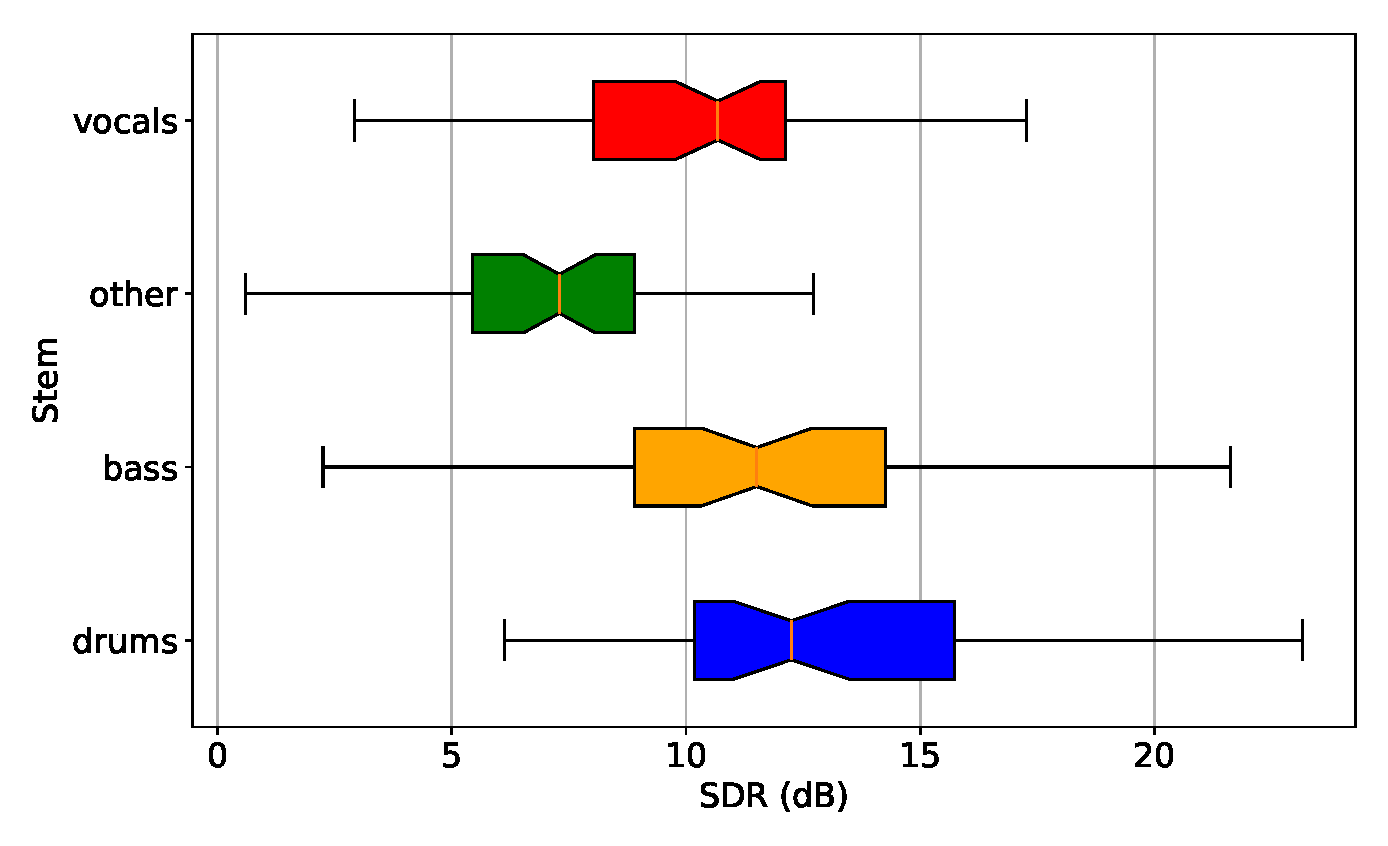
\includegraphics[width=\columnwidth]{images/box_plot_sdr_results_sdr_results.eps}}
  \caption{Evaluation of the SDR of the stems demixed by the HDemucs model in the standard usage.}
  \label{fig:sdr_results}
\end{figure}

For what it concerns the oracle predictor demonstration, the results are reported in Fig.~\ref{fig:oracle_predictor}. It can be seen that the average SI-SDR value of the target stem (``vocal'' in this case) increases, while the others decrease. This is exactly what was expected.

% \begin{figure}[t]
%   \centering
%   \centerline{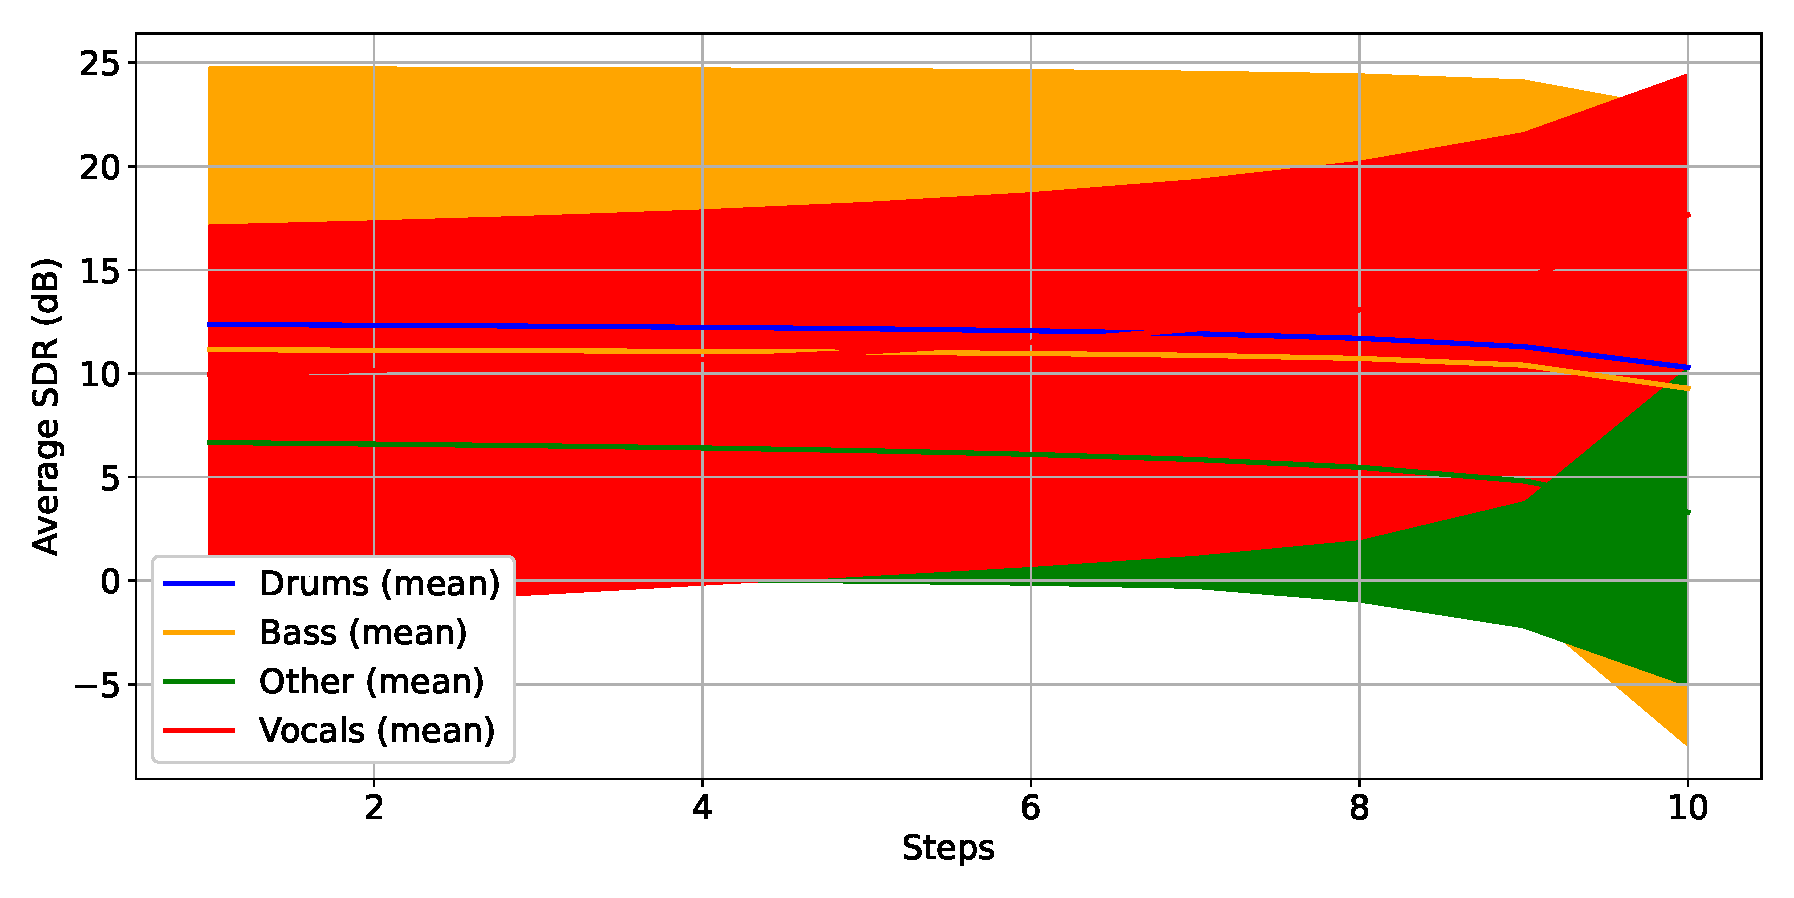
\includegraphics[width=\columnwidth]{sdr_results_oracle_predictor_sdr_results.eps}}
%   \caption{%\textcolor{red}{[CANCELLARE: lo esporta senza trasparenza se si salva in .eps, va bene anche in .png? Inoltre, meglio lasciare la didascalia così com'è o specificare in modo esplicito che si abbassano le stems dell'accompagnamento? RISPOSTA: mettiamo il png ed eventualmente prepariamo un .eps senza fill between e con linee tratteggiate e un .eps con solo le linee non tratteggiate.] DA FARE} 
%   SDR of the four stems when the relative gain of the target stem is increased for each epoch (oracle predictor).}
%   \label{fig:oracle_predictor}
% \end{figure}

\begin{figure}[t]
  \centering
  \centerline{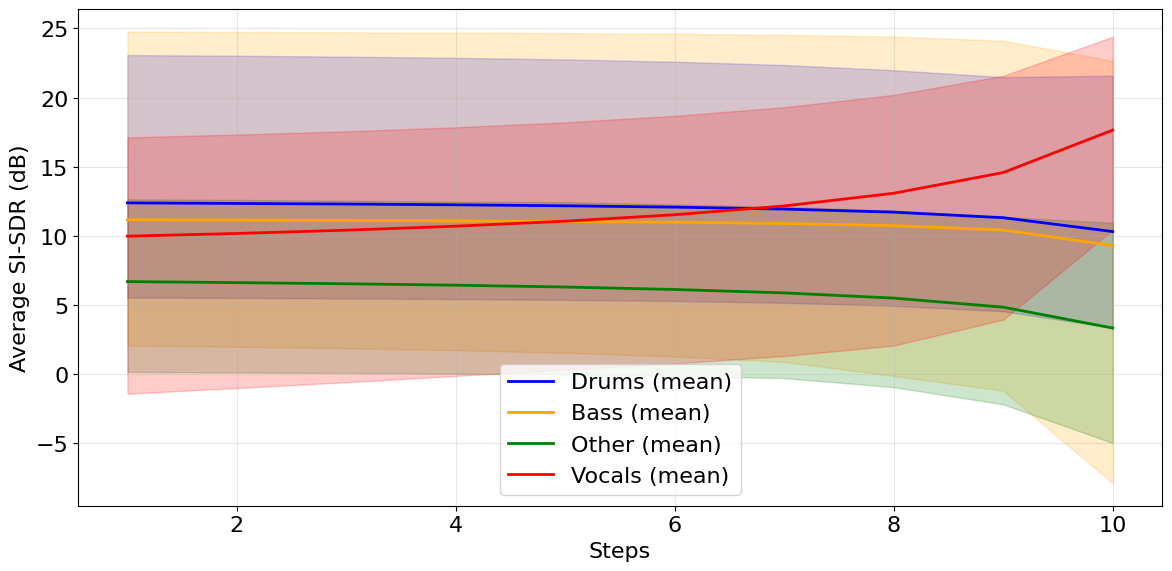
\includegraphics[width=\columnwidth]{images/si_sdr_results_oracle_predictor.png}}
  \caption{
  SI-SDR of the four stems when the relative gain of the target stem is increased for each epoch (oracle predictor).}
  \label{fig:oracle_predictor}
\end{figure}

However, the final results of the progressive inference model show that this approach is not optimal to perform this kind of operation, as shown in Fig.~\ref{fig:add_sources}. In fact, after a small improvement of the SI-SDR of the target stem for the first two iterations, the trend starts to slightly decrease. Furthermore, even the application of a Wiener filter block after every extraction did not improve the results differently from what happened to Plaja-Roglans \cite{Plaja-Roglans_2022}.
By selecting another stem as target stem, the results are similar.

% \begin{figure}[t]
%   \centering
%   \centerline{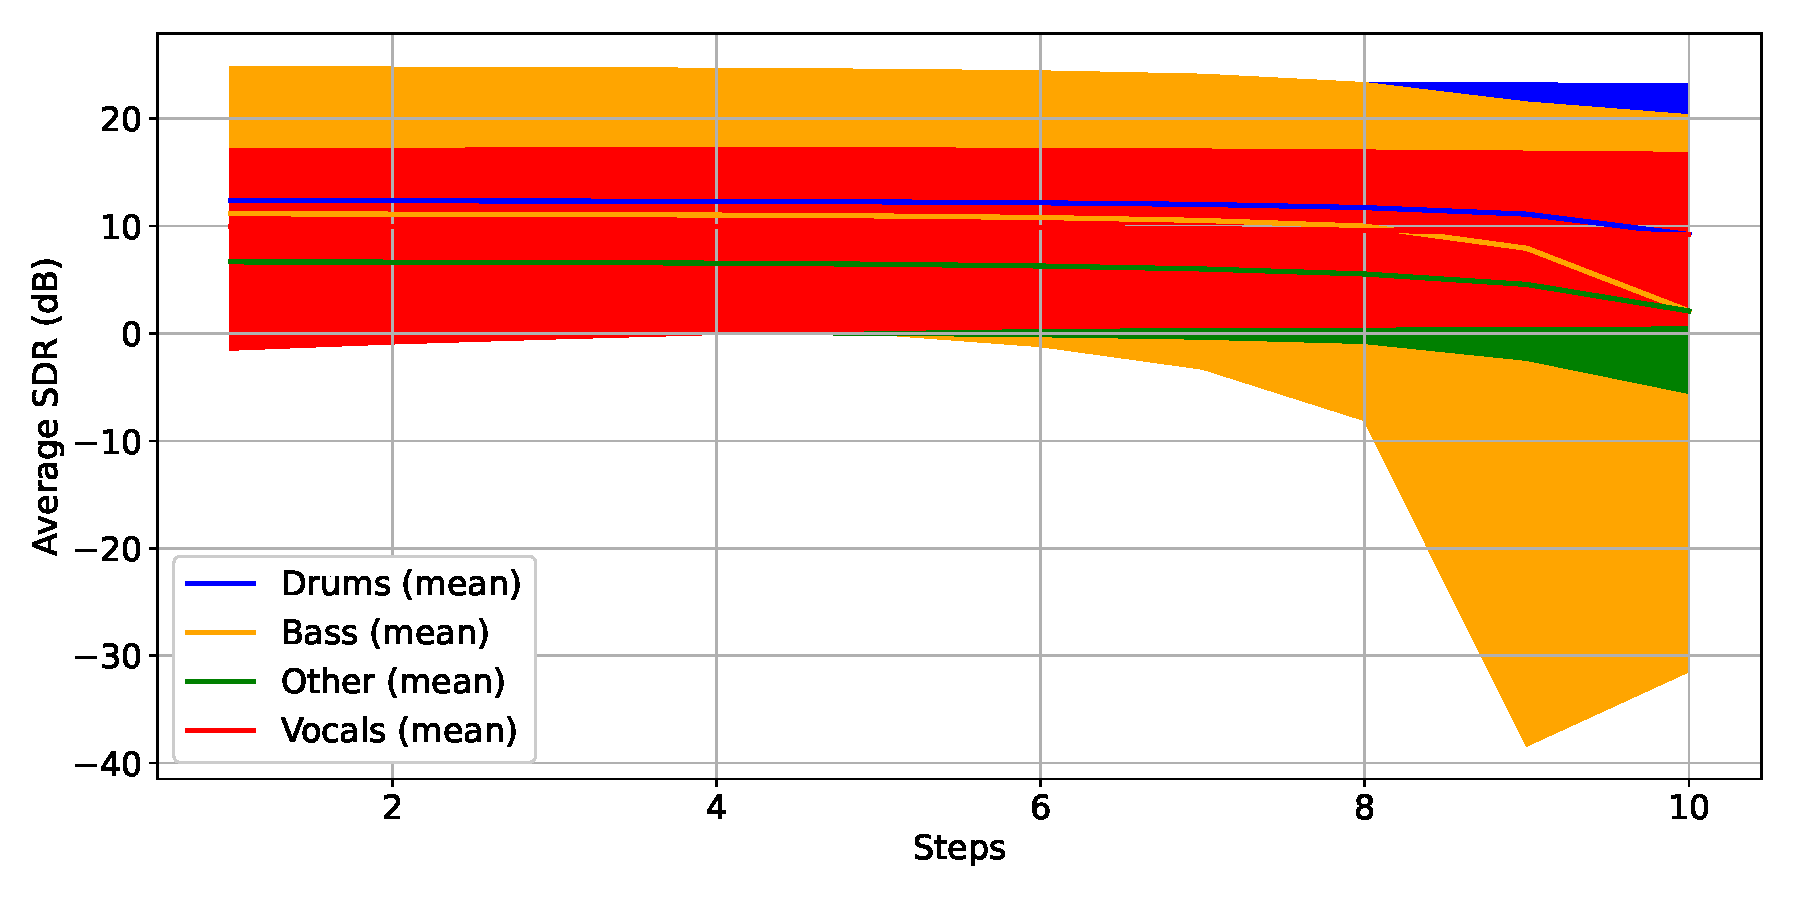
\includegraphics[width=\columnwidth]{sdr_results_add_sources_sdr_results.eps}}
%   \caption{SDR of the target stem for each epoch.}
%   \label{fig:add_sources}
% \end{figure}

\begin{figure}[t]
  \centering
  \centerline{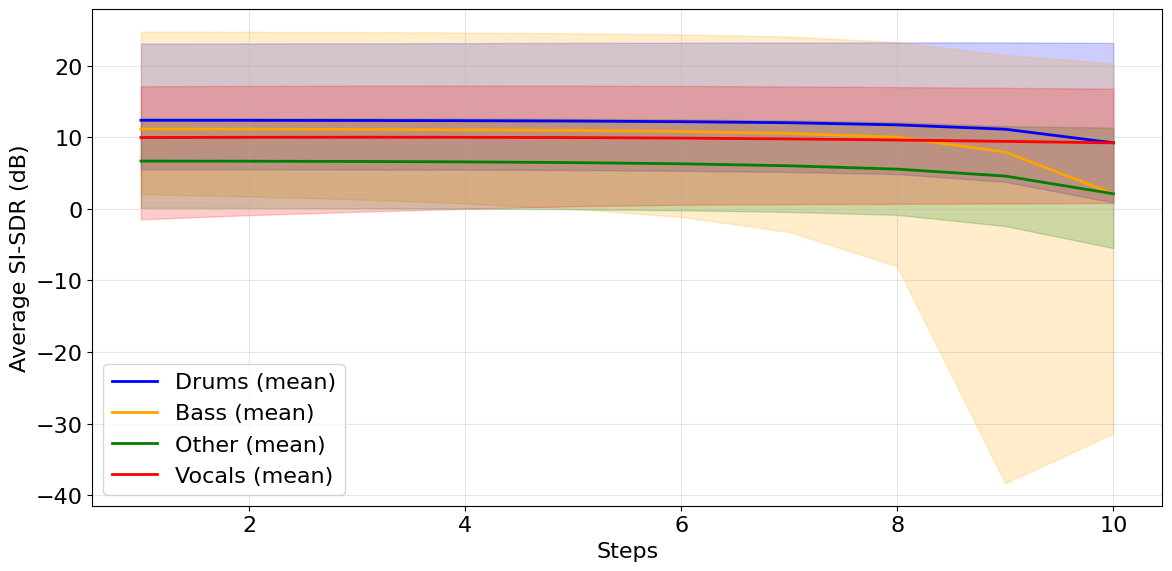
\includegraphics[width=\columnwidth]{images/si_sdr_results_add_sources.png}}
  \caption{SI-SDR of the target stem for each epoch.}
  \label{fig:add_sources}
\end{figure}

Our iterative remixing procedure – where we simply mixed the previous estimate back into the original mixture with a fixed $\beta$ schedule – did not appreciably improve separation.

In hindsight, our approach lacked several components that appear to be central in recent diffusion-based methods. For instance, Zang et al. \cite{Zang} suggest that adaptively choosing the mixing parameter $\beta$ at each step, based on a quality metric, can improve separation performance iteratively. Similarly, Plaja-Roglans et al. \cite{Plaja-Roglans_2022} train a network end-to-end with a denoising objective inspired by diffusion, progressively transforming a mixture into the target source via a learned Markov chain – achieving strong results on MUSDB18. In contrast, our method employed a fixed $\beta$ and no model retraining, offering no way for the system to adapt or refine its own outputs across iterations.

Looking forward, we believe it might be fruitful to explore whether introducing noise injection and training the model to denoise over multiple steps – as in denoising diffusion models \cite{Plaja-Roglans_2022} – could lead to more effective remixing strategies. Instead of deterministically reusing the previous estimate, the system could be trained to interpret the mixture as a noisy version of the target and gradually clean it. Recent work by Karchkhadze et al. \cite{Karchkhadze2024Improving} also points toward promising directions: they integrate a score-based diffusion model within a source separation pipeline and apply consistency distillation to reduce sampling steps, achieving strong performance gains. Whether elements of this framework – such as consistency objectives or metric-driven guidance – could help our remixing approach converge in fewer steps is an open question worth exploring.

Overall, the recent literature offers several intriguing ideas. Future work could investigate whether adaptively tuning $\beta$ (as in Zang et al. \cite{Zang}) or fine-tuning a separator like HDemucs within a denoising framework (as in \cite{Plaja-Roglans_2022}) helps structure the iterative remixing process more effectively. Likewise, training with consistency constraints (as proposed by Karchkhadze et al. \cite{Karchkhadze2024Improving}) might enable fast, diffusion-like refinement in just a few steps.

It is also possible that the effects of our proposed remixing strategies – such as fixed-step iteration or simple blending heuristics – might be more noticeable when applied to a simpler baseline model than HDemucs. Given its strong one-shot performance, HDemucs may leave limited room for iterative refinement to visibly improve results. Applying the same remixing ideas to lighter models such as Spleeter \cite{Hennequin2020Spleeter} (Deezer’s open-source separator), Conv-TasNet \cite{Luo2019ConvTasNet}, or a basic U-Net-based architecture could help assess whether the lack of improvement is intrinsic to the remixing procedure or masked by the high capacity and robustness of a state-of-the-art model.
While we have not tested these possibilities, they offer intuitions that may guide more effective designs in the future.


%\textcolor{red}{[CANCELLARE: in quest'ultima conclusione facciamo forse il passo più lungo della gamba consigliando cose che neanche abbiamo testato? RISPOSTA. chiedi a chatGPT di essere meno deciso nel consigliare l'approcio] Aggiungere tutta la parte in cui si dice che la nostra tecnica averebbe potuto dare risultati migliori se avessimo usato un modello meno potente.}


% \section{Formatting your paper}
% \label{sec:format}

% All manuscripts must be submitted electronically as PDF files. 
% All manuscripts must be formatted for white US letter paper 
% (8.5 $\times$ 11 inches). Please do {\bf not} use A4-size papers. 
% All printed material, including text, illustrations, and charts, 
% must be kept within a print area of 7.0 inches (178 mm) wide 
% by 8.9 inches (226 mm) high. Do not write or print anything outside 
% the print area. The top margin must be 1 inch (25 mm), except for 
% the title page, and the left margin must be 0.75 inch (19 mm).  
% All {\it text} must be in a two-column format. Columns are to be 
% 3.29 inches (83.5 mm) wide, with a 0.31 inch (8 mm) space between 
% them. Text must be fully justified. 



% \section{NUMBER OF PAGES}
% \label{sec:pagelimit}

% You are allowed a total of 5 pages for your document. Up to 4 pages may 
% contain technical content, figures, and references, while the 5th page 
% may contain only references. This is the max-imum number of pages that 
% will be accepted, including all figures, tables, and references. Any 
% documents that exceed the 5-page limit will be rejected. Any documents 
% with a 5th page containing anything other than references will be rejected.


% \section{PAGE TITLE SECTION}
% \label{sec:pagestyle}

% The paper title (on the first page) should begin 0.98 inches 
% (25 mm) from the top edge of the page, centered, completely 
% capitalized, and in Times 14-point, boldface type.  
% The authors' name(s) and affiliation(s) appear below the title
% in capital and lower case letters.  Papers with multiple authors 
% and affiliations may require two or more lines for this information.

% \section{TYPE-STYLE AND FONTS}
% \label{sec:typestyle}


% In nine point type font, capital letters are 2 mm high.  
% {\bf If you use the smallest point size, there should be 
% no more than 3.2 lines/cm (8 lines/inch) vertically.}  
% This is a minimum spacing; 2.75 lines/cm (7 lines/inch) 
% will make the paper much more readable. Larger type sizes 
% require correspondingly larger vertical spacing. Please do 
% not double-space your paper. True-Type 1 fonts are preferred.

% The first paragraph in each section should not be indented, 
% but all the following paragraphs within the section should 
% be indented as these paragraphs demonstrate.

% \section{SECTION TITLE}
% \label{sec:majhead}

% Major headings, for example, ``1. Introduction'', should 
% appear in all capital letters, bold face if possible, 
% centered in the column, with one blank line before, 
% and one blank line after. Use a period (``.'') after 
% the heading number, not a colon.

% \subsection{Subsection Title}
% \label{ssec:subhead}

% Subheadings should appear in lower case (initial word 
% capitalized) in boldface. They should start at the left 
% margin on a separate line. 
 
% \subsubsection{Sub-subsection Title}
% \label{sssec:subsubhead}

% Sub-subheadings, as in this paragraph, are discouraged. 
% However, if you must use them, they should appear in 
% lower case (initial word capitalized) and start at the 
% left margin on a separate line, with paragraph
% text beginning on the following line. They should be 
% in italics. 
 

% \section{ILLUSTRATIONS, GRAPHS, AND PHOTOGRAPHS}
% \label{sec:illust}

% Illustrations must appear within the designated margins.  
% They may span the two columns. If possible, position 
% illustrations at the top of columns, rather than in 
% the middle or at the bottom. Caption and number every 
% illustration. All halftone illustrations must be clear 
% black and white prints. Colors may be used, but they 
% should be selected so as to be readable when printed 
% on a black-only printer.

% Since there are many ways, often incompatible, of 
% including images (e.g., with experimental results) 
% in a \LaTeX\ document, an example of how to do
% this is presented in Fig.~\ref{fig:sdr_results}.

% Below is an example of how to insert images. 
% -------------------------------------------------------------------------



% \section{Equations}
% \label{sec:equations}

% Equations should be placed on separate lines and consecutively
% numbered with equation numbers in parentheses flush with the 
% right margin, as illustrated in (\ref{eqn:wave_equation}) 
% that gives the homogeneous acoustic wave equation in
% Cartesian coordinates \cite{eWilliams1999},
% \begin{equation}
%   \label{eqn:wave_equation}
%     \Delta^2p(x,y,z,t)-
%     \displaystyle\frac{1}{c^2}\frac{\partial^2p(x,y,z,t)}{\partial t^2}=0,
% \end{equation}
% where $p(x,y,z,t)$ is an infinitesimal variation of acoustic 
% pressure from its equilibrium value at position $(x,y,z)$ and 
% time $t$, and where $c$ denotes the speed of sound.

% Symbols in your equation should be defined before the equation 
% appears or immediately following.  Use (1), not Eq. (1) or 
% equation (1), except at the beginning of a sentence:  
% ``Equation (1) is ...''



% \section{FOOTNOTES}
% \label{sec:foot}

% Use footnotes sparingly (or not at all!) and place them at 
% the bottom of the column on the page on which they are 
% referenced. Use Times 9-point type, single-spaced. To 
% help your readers, avoid using footnotes altogether and
% include necessary peripheral observations in the text 
% (within parentheses, if you prefer, as in this sentence).


% \section{REFERENCES}
% \label{sec:ref}

% List and number all bibliographical references at the end 
% of the paper. The references should be numbered in order 
% of appearance in the document. When referring to them in 
% the text, type the corresponding reference number in 
% square brackets as shown at the end of this sentence 
% \cite{cJones2003}, \cite{aSmith2000}. For \LaTeX\ users, 
% the use of the Bib\TeX\ style file IEEEtran.bst is 
% recommended.

% \section{ACKNOWLEDGMENT}
% \label{sec:ack}

% The preferred spelling of the word acknowledgment in 
% America is without an ``e'' after the ``g.'' Try to avoid 
% the stilted expression, ``One of us (R. B. G.) thanks ...''
% Instead, try ``R.B.G.\ thanks ...''  Put sponsor 
% acknowledgments in the unnumbered footnote on the first page.

% -------------------------------------------------------------------------
% Either list references using the bibliography style file IEEEtran.bst
%\newpage [CANCELLARE]
\clearpage
\bibliographystyle{IEEEtran}
\bibliography{refs21}
%
% or list them by yourself
% \begin{thebibliography}{9}
% 
% \bibitem{waspaa21web}
%   \url{http://www.waspaa.com}.
%
% \bibitem{IEEEPDFSpec}
%   {PDF} specification for {IEEE} {X}plore$^{\textregistered}$,
%   \url{http://www.ieee.org/portal/cms_docs/pubs/confstandards/pdfs/IEEE-PDF-SpecV401.pdf}.
%
% \bibitem{PDFOpenSourceTools}
%   Creating high resolution {PDF} files for book production with 
%   open source tools, 
%   \url{http://www.grassbook.org/neteler/highres_pdf.html}.
%
% \bibitem{eWilliams1999}
% E. Williams, \emph{Fourier Acoustics: Sound Radiation and Nearfield Acoustic
%   Holography}. London, UK: Academic Press, 1999.
% 
% \bibitem{ieeecopyright}
%   \url{http://www.ieee.org/web/publications/rights/copyrightmain.html}.
%
% \bibitem{cJones2003}
% C. Jones, A. Smith, and E. Roberts, ``A sample paper in conference
%   proceedings,'' in \emph{Proc. IEEE ICASSP}, vol. II, 2003, pp. 803--806.
% 
% \bibitem{aSmith2000}
% A. Smith, C. Jones, and E. Roberts, ``A sample paper in journals,'' 
%   \emph{IEEE Trans. Signal Process.}, vol. 62, pp. 291--294, Jan. 2000.
% 
% \end{thebibliography}


\end{sloppy}
\end{document}
